\chapter{Software differential patching}
With the new binary versions generated by UCC technique, I define a update script format to summarize the code 
difference between the base binary and the newly generated binary. The framework then will transmit the patch script to 
the sensors, and let the sensors reconstruct the new binary. As shown in Figure~\ref{patch}, the old version binary 
\texttt{E} and the new version binary \texttt{E'} are first compared, and then the binary level differences are 
formatted as the update script \texttt{U}. After the sensors receive the complete \texttt{U}, they will retrieve the 
new binary image \texttt{E'} by combining \texttt{U} with the old binary image \texttt{E} which already exists in the 
sensor memory.

\begin{figure}[htbp]
\centering
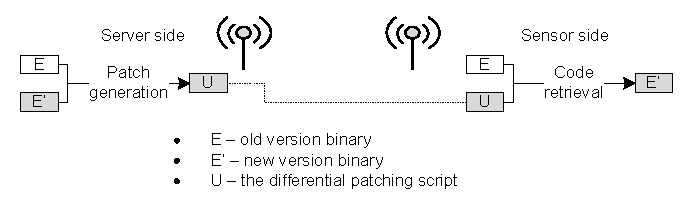
\includegraphics[scale=1.2]{figures/patch.eps}
\caption{Patch generation and binary reconstruction.}
\label{patch}
\end{figure}


The binary code may be changed due to functionality change or data layout change, thus, I separate these two kinds of 
changes in the update script, as the functional script part and data layout part representatively.
The design of the script primitives affects both the update data packet transmission effectiveness and the runtime 
overhead on each sensor node. To facilitate the description of UCC techniques, I adopted four simple code update 
primitives from the prior work~\cite{related:script}, and propose three advanced functional primitives and three data 
layout primitives to describe the higher level code changes. 

\section {Instruction based patching}

I use the functional binary update primitives to describe the functional changes, such as adding, removing or updating 
instructions caused by functionality changes. 
I adopted the simple primitives from the prior work~\cite{related:script} and proposed the advanced primitives to solve 
more complicated code compression problems. The difference between the advanced primitives and the simple primitives is 
that they are not used to describe the simple bit level comparison results, but higher level structure changes such as 
the destination address shifting for a group of instructions.

The format of the script primitives is shown in Figure~\ref{fscript}. 

\begin{figure}[htbp]
\centering
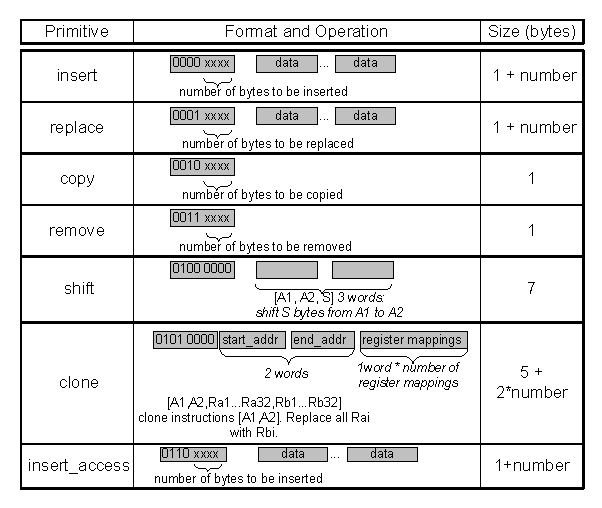
\includegraphics[scale=1.2]{figures/fopcode.eps}
\caption{The functional patch script primitives}
\label{fscript}
\end{figure}


\subsection{Simple primitives}

There are four simple primitives --- {\tt insert}, {\tt replace}, {\tt copy}, and {\tt remove}. Both {\tt insert} and 
{\tt replace} primitives have one-byte opcode and {\tt n} bytes of data/instructions to be incorporated.  The {\tt 
copy} and {\tt remove} primitives take one byte each and specify the size of old data/instruction block to be
copied or removed.

\begin{figure}[htbp]
\centering
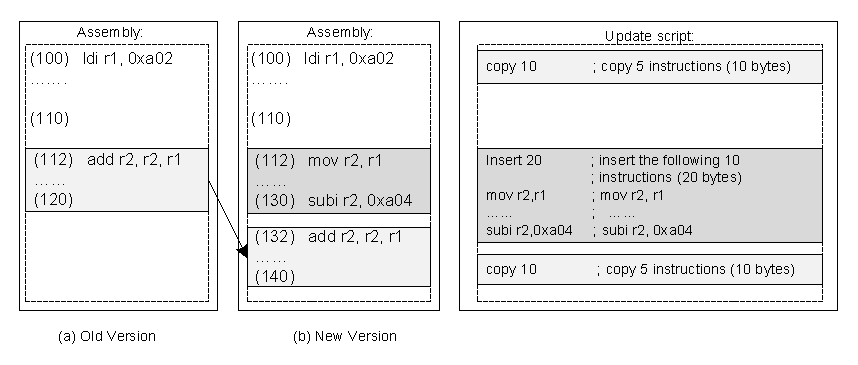
\includegraphics[width=6in]{figures/sother.eps}
\caption[An example of the simple primitives.]{An example of the simple primitives. 
New code {\tt [112,130]} is inserted.
{\tt [112,120]} in the original code is now moved to {\tt [130,140]} 
in the new version.
}
\label{fsother}
\end{figure}

Figure \ref{fsother} shows an example of the simple primitives. The new version contains three chunks of code, {\tt 
[100,110]}, {\tt [112,130]}, and {\tt [132,140]}. Both the first and third chunks can be found in the old code while 
the second chunk is new. Therefore the update script contains two {\tt copy} primitives and one {\tt insert} primitive. 
The {\tt insert} primitive has a one-byte opcode and ten instructions (or 20 bytes). The total size of the update 
script is 23 bytes.  

In order to interpret the simple primitives on remote sensors,
the script interpreter maintains two instruction pointers, one points to the old
binary image and the other points to the last instruction that has been generated
in the new binary image. 
The {\tt insert} primitive inserts the instructions
in its data part into the new binary image, and moves the pointer in the
new code to the end. The {\tt replace} primitive does the same thing to
the new binary but also moves the pointer in the old binary for the
same distance. The {\tt copy} primitive reads the instructions from the
old binary, and moves both pointers.
 
\subsection {Advanced primitives}
In the experiment, I observed some code structure changes that affect more than one instruction. For example, when the 
register assignment of one variable is different in the new binary, all the instructions that access this variable need 
to be updated. Since the affected instructions are usually more than one, it is cheaper to incorporate such register 
assignment changes in the patch script, other than the binary level differences. Based on this observation, I propose 
three advanced primitives in my design.

\subsubsection {shift}
As some code may be inserted into or removed from the base binary in software update, the absolute address of the 
instructions may be changed in the update. Such change might cause the destination address changes for branch 
instructions.  I use the {\tt shift} primitive~\cite{related:script} that informs the sensors about the destination 
address shifts, so that the sensors can incorporate such code changes on side. Instead of explicitly updating all the 
affected branch instructions using several {\tt update} primitives, now we can use one  {\tt shift} primitive to 
describes such code changes. The update script size can be significantly reduced. 

As Figure~\ref{fscript} shows, the {\tt shift} primitive contains a one-byte opcode and another three words to indicate 
that
the code segment {\tt [A1,A2]} is now moved to {\tt [A1+S,A2+S]}. All the branch/jump instructions whose destination 
addresses are in the range {\tt [A1,A2]}, will have the destination addresses shifted by {\tt S} on the sensor side.

%To interpret the {\tt shift} script, the binary rewriter running on the sensor nodes needs to have simple decoding 
ability --- it picks up each control transfer instruction, checks whether its target address falls in the range that 
needs to be shifted, and updates them with new addresses.
%For absolute branch instructions, their target addresses can be decoded from the instruction directly; for relative 
branch instructions, their target addresses can be computed by adding the relative offset to the address of the current 
instruction.

\begin{figure}[htbp]
\centering
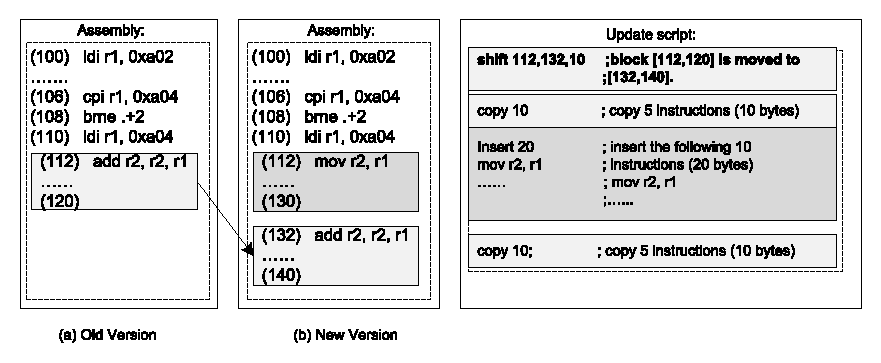
\includegraphics[width=6in]{figures/shift.eps}
\caption[An example of the {\tt shift} primitive.]{An example of the {\tt shift} primitive. New code {\tt [112,130]} is 
inserted. {\tt [112,120]} in the old code is now moved to {\tt [132,140]} 
in the new version. Some control flow instructions are affected due to this address change.
}
\label{fshift}
\end{figure}

Figure \ref{fshift} shows an example of the {\tt shift} primitive. Due to the insertion of
new code, the chunk {\tt [112,120]} in the old version is now moved to {\tt [132,140]} 
in the new version. All the branch instructions that
jump to any instruction inside this chunk need to be updated. In the example, the {\tt shift} primitive
specifies that all the branch instructions whose targets are in the address range {\tt [112,120]} should be shifted by 
20. 

When one block movement causes several changes in the code, using the {\tt shift} primitive helps to reduce the script 
size. The tradeoff is that a slightly more powerful interpreter has to be installed on the sensor side such that it can 
decode each instruction type to extract the desired target address. 

The sensors will interpret the {\tt shift} primitive in the following way. 
For the absolute branch instructions, the original destination is decoded
first and if it falls in the shift range, it will be updated according
to the offset encoded in the primitive.
For the relative branch instructions, their target addresses can be computed by adding the relative offset to the 
address of the current instruction.

It is implemented by maintaining a shift information table. When encountering a {\tt shift} primitive,
one shift entry is added to the table, which includes the start address, end address and shift offset.
When copying one instruction from the old binary to the new binary, the interpreter will check this table to see if it 
is a branch or jump instruction. If the target address falls in any shifting range, the destination of this instruction 
will be updated.
%\begin{figure}[htbp]
%\begin{center}
%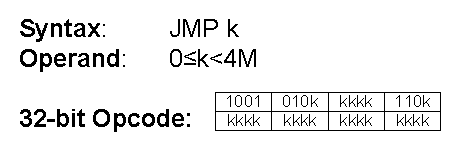
\includegraphics[width=2.2in]{./figures/jump.eps}
%\caption{{\tt JMP} instruction in AVR instruction set.
%}
%\label{jump}
%\end{center}
%\end{figure}
%For example, in the AVR instruction set~\cite{avr-inst}, {\tt JMP} instruction updates the
%the program counter to make the execution ``jump'' to the destination.
%The format is shown in Figure~\ref{jump}. The sample code below shows
%how to update the destination address for {\tt JMP} instructions.
%\begin{algorithmic}
%\singlespace
%\IF {$*(P_{old})$ AND 0xfe0e $\neq$ 0x940c} 
%        \STATE old\_dest = (($*P_{old}$ AND 0x01f0) $\gg$ 3 )+  ($*P_{old}$ AND 0x1);
%        \STATE old\_dest $<$= 16;
%        \STATE old\_dest += $*(P_{old}+1)$;
%        \IF {old\_dest $\in$ {shift range}}
%        
%        	\STATE new\_dest = old\_dest + offset;
%        	\STATE new\_inst = 0x940c;
%       	 	\STATE new\_inst\_high $|$= (new\_dest $\gg$16 ) AND 0x1;
%        	\STATE new\_inst\_high $|$= ((new\_dest $\gg$16) AND 0x3e) $\ll$ 3; 
%        	\STATE new\_inst\_low = (new\_dest AND 0xffff);
%        \ENDIF
%\ENDIF 
%\end{algorithmic}

\subsubsection {clone}
In the experiments, I found that the binary code of the {\tt inline} functions called at different locations looks very 
similar with each other, although different register are used. This is because they are compiled from the same source 
code, however, due to the different context, different register assignment decisions may be made. Although they only 
differ in the register usages, when an {\tt inline} function is introduced or updated, similar copies are inserted or 
updated more than once in the binary, which is a waste.

Based on this observation, I introduced the {\tt clone} primitive. 
When an {\tt inline} function is inserted or modified in the code update, the update script only includes one copy of 
the binary generated by the {\tt inline} function, and advises the sensors to 
replicate the master copy with register usage replacement while constructing the binary for the other instances of this 
{\tt inline} function.

The example below shows how the {\tt clone} primitive works.
Assume that an {\tt inline}
function is called at multiple locations, such as block {\tt [A1,A2]} and {\tt [B1,B2]}. 
The patch generator uses block {\tt [A1,A2]} as the comparison base, 
and tries to match the register allocation between these two blocks. 
Assume the register mapping between them is shown as below, 
$(\it{R_{a1},R_{a2},...,R_{an})\Rightarrow(R_{b1}^\prime,R_{b2}^\prime,...,R_{bn}^\prime)}$.
Given such information, instead of using a sequence of the simple primitives to describe the
updated/new code of block {\tt [B1,B2]}, we could rather copy instructions from block 
{\tt [A1,A2]}, and slightly change the register
assignments according to the register mapping 
to rebuild block {\tt [B1,B2]}.


As shown in Figure~\ref{fscript},The {\tt clone} primitive has one-byte opcode, and another
several bytes to specify the starting and ending address 
of the code segment where the code would be copied from, and the register mappings.
The primitive length varies according to the register mapping complexity.
Assume there are {\tt N} pairs of register mappings, the {\tt clone} primitive length is
{\tt 5+2*N}. An {\tt inline} function may have multiple instances in the binary image. The 
instance that is stored with the lowest addresses will be considered as the master copy.
The other instances will clone the code from the master copy.


Figure \ref{fclone} shows an example using the {\tt clone} primitive.  Both the code {\tt [200,206]} and 
{\tt [100,106]} are compiled from the same {\tt inline} function. Instead of generating the update script for 
{\tt [200,206]} by using the {\tt insert} primitive, the {\tt clone} primitive is used to specify that the second code block 
clones the block {\tt [100,106]} while registers  
${\tt r_1}$ and ${\tt r_2}$ needs to be updated to be ${\tt r_{11}}$ and ${\tt r_{12}}$ respectively.
\begin{figure}[htbp]
\centering
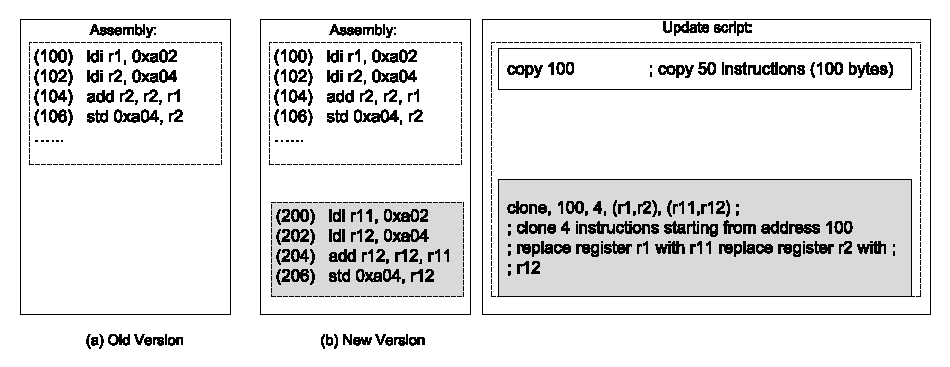
\includegraphics[width=6in]{figures/sclone.eps}
\caption[An example of the {\tt clone} primitive.]{An example of the {\tt clone} primitive. New code {\tt [200,206]}, 
which
is compiled from the same {\tt inline} function as code {\tt [100,106]} is inserted.}
\label{fclone}
\end{figure}

The {\tt clone} primitive can reduce the script size when the {\tt inline} function is
called at multiple places, and the register mapping is clear. However, if the register mapping
is too complicated the script size could be very big, in which case it is better to use the simple primitives, such as 
{\tt insert} and {\tt replace}. In addition, it requires the sensor-side interpreter to have simple decoding ability to 
extract register names from different instruction types, and replace them with new ones. 
The sensors need to reconstruct the code segment
by replacing the registers in the master copy according to the patch script.
Each clone operation will need to decode the instructions in the master copy and
replace the registers. Thus, when the master copy is frequently cloned, it is more
efficient to store the master copy in a storage buffer and add tags
to each instruction indicating whether this is a memory access instruction and
which register is used, so that the clone process can speed up.

%In order to interpret the {\tt clone} primitive, the sensor needs to scan the update script twice.
%In the first scan, it builds the clone information table, which includes the start
%and end address of the master copy and the number of clone operations.

%In the second scan, when the new code pointer encounters the master copy, 
%the code segment will be stored in the buffer until all its clone
%operations are complete. The related entry in the clone information table 
%is updated to record the location of the code segment in the buffer.

%When interpreting a {\tt clone} primitive, the
%sensor will look up the clone information table to locate the code segment in
%the buffer, copy it and replace the registers according to the script.
%The clone counter in the information table keeps track of the number of 
%clones that need to be done. Once it reaches zero,
%the buffer used to store the master copy will be released. 
%Figure~\ref{cloneexample} shows the interpretation
%procedure of the example given in Figure~\ref{fclone}.

%\begin{figure}[htbp]
%\centering
%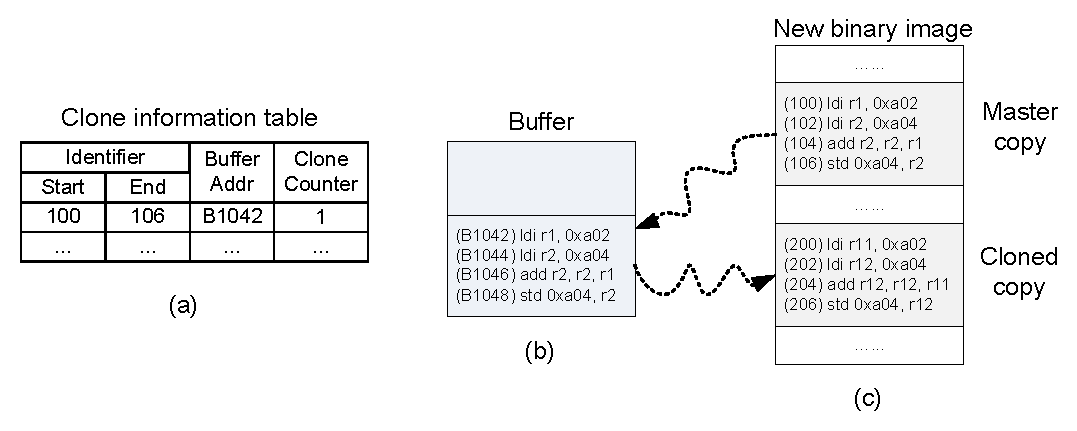
\includegraphics[width=5in]{./figures/clone.eps}
%\caption{An example of the {\tt clone} primitive interpretation procedure.
%(a). The clone information table. (b). The buffer. (c). The 
%reconstructed binary image.}
%\label{cloneexample}
%\end{figure}

%For the frequently cloned master copies, tags can be added to the instructions stored in 
%the buffer to mark the register usage, such that we do not have to decode
%each instruction to detect the old register assignment and replace that with the
%corresponding new one.
%A fast register replacement can be achieved.


\subsubsection{insert\_access}

When inserting a new memory access between two existing accesses, we may need two {\tt replace} primitives and one {\tt 
insert} primitive, as shown in Figure \ref{insacc}(d). Since the update primitives only modify the addressing modes, a 
compact way to express it is to include the memory address difference in the script and let the mobile devices generate 
the correct addressing modes for the related instructions. Thus, I introduce an {\tt advanced primitive} -- 
{\tt insert\_access}.

\begin{figure}[htbp]
\begin{center}
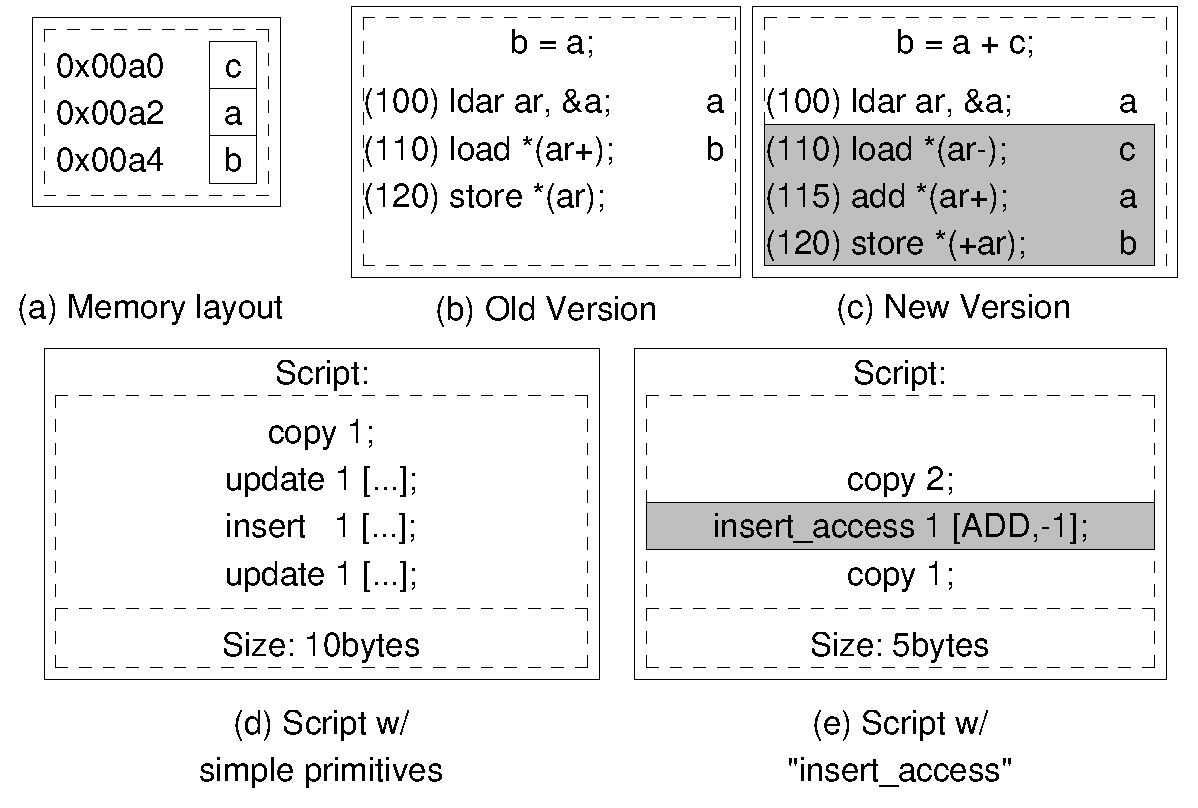
\includegraphics[width=4in]{./figures/insacc.eps}
\caption[An example of the {\tt insert\_access} primitive.]{An example of the {\tt insert\_access} primitive:
(a) The memory layout for both versions;
(b) The source and assembly before code update;
(c) The  source and assembly after code update;
(d) The update script using the simple primitives;
(e) The update script using the {\tt insert\_access} primitives.
}
\vspace{-0.5in}
\label{insacc}
\end{center}
\end{figure}

The {\tt insert\_access} primitive is similar to the {\tt insert} primitive, except that its data field is specified as 
follows:
\begin{eqnarray}
[\textit{operation},\delta_{\textit{diff}}]\nonumber
\end{eqnarray}
where $\delta_{\textit{diff}}$ represents the address difference between the locations accessed by the current 
instruction and the preceding instruction respectively. In the example (Figure \ref{insacc}(c)), the new access is
 {\it c }(located in memory slot 0), and the preceding memory access is {\it a} (located in memory slot 1), so 
$\delta_{\textit{diff}}$ is -1.
Since it is the add operation that accesses {\tt c} in the new instruction, the update primitive is  
\begin{eqnarray}
 \texttt{insert\_access} ~~~1 ~~ [\tt{ADD}, -1].\nonumber
\end{eqnarray}

Rewriting the update script of the example, using the {\tt insert\_access} primitive, the script size is reduced by 
50\% (Figure \ref{insacc}(e)). 

The {\tt insert\_access} primitives allows the sensors to correct the
addressing modes before and after the newly inserted memory access.

Let us call the last memory access instruction before the inserted instruction the {\tt 
predecessor} and the first one that is executed after the inserted instruction the
{\tt successor}.
Based on these two instructions, the offset between them can be calculated.
The {\tt insert\_access} primitive encodes the offset between the inserted
memory access and the {\tt predecessor}, thus the offset between each two 
instructions among these three can be calculated.
Based on that information, the addressing modes can be determined.

\begin{figure}[htbp]
\centering
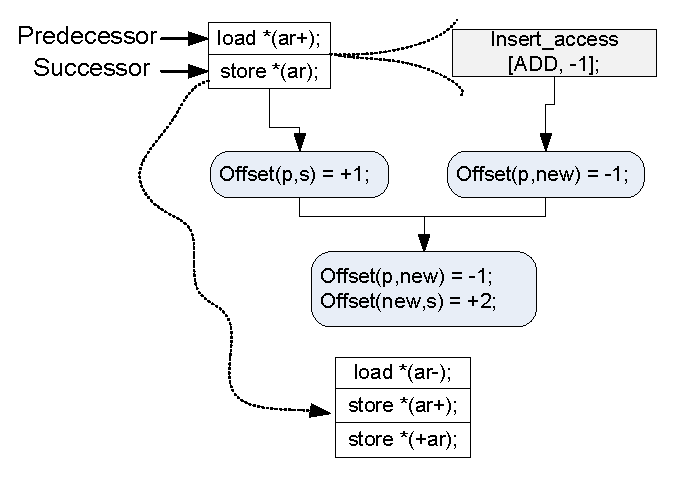
\includegraphics[width=3.5in]{./figures/insert_access.eps}
\caption{An example of the interpretation procedure of the {\tt insert\_access} primitive .}
\label{insertaccess}
\end{figure}

Figure~\ref{insertaccess} demonstrates the interpretation procedure of the
example given in Figure~\ref{insacc}. Knowing the offset between the {\tt predecessor}
and the inserted instruction is -1, and the offset between the inserted
instruction and the {\tt successor} is +2, the addressing mode of the 
{\tt predecessor} can be determined to be pre-incremental, that of the inserted
instruction can be determined to be post-incremental and that of the
{\tt successor} can be determined to be pre-incremental.

\subsection{Sensor-side interpretation for functional primitives}

The received patch scripts will be stored in the program memory.
When the script download is complete, the sensors will run a simple script
interpreter to incrementally reconstruct the new binary image.
The reconstruction is based on the received the patch script and
the old binary image which is stored in the program flash on the
sensors.
The generated new binary image will be stored in the program flash as well.
When the primitive interpretation is complete, the sensors will load
the new binary image back to the program memory and restart
to execute the new version.
The old image will be kept in the program flash until the space is 
needed to store newer versions, so that when an execution error
happens, the sensors can roll back to the older version.
However, because sensors use cyclic redundancy check (CRC) to ensure the data integrity
while transmitting the patch messages, and the reconstruction
has been tested on the server side to make sure that it can generate
the correct binary image, there is a very small chance that the
new binary image is not functioning correctly.


The flash memory used to store both the old and new binary images
can be read in a random access fashion, so the pointer that is pointing
to the old binary can be moved arbitrarily when it is needed.
However, one limitation of the flash memory is that it has to be programmed 
at block levels, e.g. 256 bytes on for mica2 sensors~\cite{mica2-power}.
In order to change one byte, the sensor has to read the correspond block into
program memory, modify it and then write it back.
Thus, the constructed new binary needs to be buffered in the program memory
first until it reaches the size of a flash block, then the code block will be
written back to the program flash. The size of the temporary code buffer 
should be a multiplier of the block size.


The interpretation algorithm is presented in Algorithm~\ref{decode}.
Each script primitive is scanned once, and is interpreted to construct
the new binary. 
Besides that, the interpreter maintains two instruction pointers, one points to the old
binary image and the other points to the last instruction that has been generated
in the new binary image. 

To interpret the  {\tt insert} and {\tt replace} primitives, it copies the instructions from the data
part of the primitive to the new binary.  To interpret the {\tt copy} primitive, it copies
the instructions from the old binary image instead.
The two pointers are updated as well. The pointer in the new binary always
points to the end of the image. The pointer in the old binary is shifted according
to the number of bytes that have been copied, removed or updated, according to the
script.


\begin{algorithm}
\singlespace
\begin{algorithmic}[1]
\singlespace
\REQUIRE{ Pointer to the beginning of the patch script $P_S$, \\
	Pointer to the beginning of the old binary $P_O$,\\ 
	Pointer to the beginning of the new binary $P_N$.}
\FOR{(; $P_S \neq {\it script}.end()$; $P_S$= {\it script}.{\it next\_primitive()})}	
	
\STATE {\bf switch}( primitive\_type($P_S$)

\STATE \hspace{5 mm} {\bf case} insert:
\STATE \hspace{10 mm} {\bf write\_code\_buffer}($P_N$, insert\_data($P_S$), insert\_bytes($P_S$))
%\STATE \hspace{10 mm} $P_N$ += insert\_bytes($P_S$);
\STATE \hspace{10 mm} {\bf break}

\STATE \hspace{5 mm} {\bf case} replace:
\STATE \hspace{10 mm} {\bf write\_code\_buffer}($P_N$, replace\_data($P_S$), replace\_bytes($P_S$))
%\STATE \hspace{10 mm} $P_N$ += replace\_bytes($P_S$)
\STATE \hspace{10 mm} $P_O$ += replace\_bytes($P_S$)
\STATE \hspace{10 mm} {\bf break}

\STATE \hspace{5 mm} {\bf case} copy:
\STATE \hspace{10 mm} {\bf write\_code\_buffer}($P_N$, $P_O$, copy\_bytes($P_S$))
%\STATE \hspace{10 mm} $P_N$ += copy\_bytes($P_S$);
\STATE \hspace{10 mm} $P_O$ += copy\_bytes($P_S$)
\STATE \hspace{10 mm} {\bf break}

\STATE \hspace{5 mm} {\bf case} remove:
\STATE \hspace{10 mm}  $P_O$ += remove\_bytes($P_S$)
\STATE \hspace{10 mm} {\bf break}

\STATE \hspace{5 mm} {\bf case} shift:
\STATE \hspace{10 mm} add $\left[ A1(P_S), A2(P_S), S(P_S)\right]$ to addr\_shift\_table
\STATE \hspace{10 mm} {\bf break}

\STATE \hspace{5 mm} {\bf case} clone:
\STATE \hspace{10 mm} {\bf if} ([start\_addr($P_S$), end\_addr($P_S$)] is not in clone\_buffer)
\STATE \hspace{15 mm} load code [start\_addr($P_S$), end\_addr($P_S$)] $\Rightarrow$  clone\_buffer;
\STATE \hspace{10 mm} {\bf endif}
\STATE \hspace{10 mm} replace\_register(buffer,register\_pairs($P_S$) )
\STATE \hspace{10 mm} {\bf write\_code\_buffer}($P_N$, buffer, clone\_bytes($P_S$))
\STATE \hspace{10 mm} {\bf break}

\STATE \hspace{5 mm} {\bf case} insert\_access:
\STATE \hspace{10mm} update the addressing mode of $P_N-1$ if necessary
\STATE \hspace{10mm} generate the addressing mode $addr\_mode$ for the inserted instruction
\STATE \hspace{10mm} instruction $i$ = form\_inst(opcode($P_S$),$addr\_mode$)
\STATE \hspace{10mm} {\bf write\_code\_buffer}($P_N, i$, length($i$))
\STATE \hspace{10mm} {\bf break}

\STATE \hspace{5mm} {\bf default}:
\STATE \hspace{10mm} error(``no such primitive'')
\STATE {\bf end switch}
\ENDFOR
\STATE copy new\_binary to program\_memory
\STATE restart the sensor
\end{algorithmic}
\caption{Primitive interpretation and code reconstruction.}
\label{decode}
\end{algorithm}

When encountering the {\tt shift} primitive, one entry that records the start address, end address
and shift offset is inserted to the shift table. To interpret the {\tt clone} primitive, the
master copy will be read from the program memory and register usage will be modified
to construct the cloned copy. The master copy needs to be read 0 to $K$ times, where
$K$ is the number of cloned copies that it has. In order to avoid reading the program
memory $K$ times, this master copy can be buffered in the program memory.
The {\tt insert\_access} primitive will decode the predecessor
and the successor to correct the addressing mode. Because the generated code is first
buffered in program memory, and there is usually one or two instructions inserted by
this primitive, both the predecessor and successor may still in the temporary code buffer.
Thus, this operation may not cause read or write to the new binary image.

When the whole code construction process is complete, the new binary image
will be copied to the program memory from the program flash. The sensor will
then restart to run the new code.


The algorithm shown in Algorithm~\ref{copycode} is called whenever a 
instruction is constructed and written to the temporary code buffer.
A simple decode operation is done first to filter out the branch instructions.
If the target address of the branch instruction falls in any range that needs address
shifting, this instruction will be updated for the address shift.
When the temporary buffer is full, the code block will be copied to the
program flash.


\begin{algorithm}
\singlespace
\begin{algorithmic}[1]
\singlespace
\REQUIRE{ Destination address \& $P_N$, \\
	Source address $P_O$,\\
	Number of bytes to be copied $nbytes$.}
\STATE memcpy($P_N$,$P_O$,$nbytes$);
\FORALL{ instructions $i$ to be copied}
	\IF {inst\_type($i$) == branch/jump}
		\STATE $target$ = target\_addr($P_N$)
		\IF {there exists a shift entry $e\in$ shift\_table, where $target\in \left[ e.A1, e.A2\right]$}
			\STATE $target = target+e.offset$
			\STATE change the target address of $P_N$ to $target$
		\ENDIF
	\ENDIF	
\ENDFOR
\STATE $P_N$ += $nbytes$
\IF {$P_N == {\it code\_buffer}.end$}
	\STATE write\_to\_flash(\it code\_buffer)
	\STATE $P_N = {{\it code\_buffer}}.begin$
\ENDIF
\end{algorithmic}
\caption{{\bf write\_code\_buffer} \/\/write the constructed code into code buffer}
\label{copycode}
\end{algorithm}

The memory space required for the interpreter include the temporary code buffer
and the shift table. As discussed before, the minimal size of the code buffer is the block
size of the program flash, which is 256 bytes for Mica2 sensor.
Each entry of the shift table includes the start address, end address and the shift offset.
As the program memory size is 4 kbytes, the start address and end address can be
encoded using 3 bytes. The shift offset can encoded using 1 byte. Thus, the storage
required for each entry is 4 bytes.


\section{Data based patching}



 I observed that binary changes at several places may be caused by one memory layout change in the experiments. 
Assuming variable {\tt a} appears in several places in the code and is relocated to a new memory location, we may 
generate a script with multiple update primitives each of which presents one instruction level change. Instead, if the 
script interpreter on mobile devices can decode DSP instructions, and identify all the uses of {\tt a}, it is possible 
to send one ``relocate {\tt a}'' primitive instead of individual instruction update. 

Let us call the binary instructions that are inserted, removed, or changed due to the offset assignment changes as {\it 
addressing mode change} (AMC) instructions. The motivation of developing {\it data primitives} is to reduce the 
transmission of AMC instructions, and let the mobile devices construct them by themselves. Compared to the 
{\it insert\_access} primitive, data primitives are designed to update the code in more than one place.

\subsection{Data update primitives}
\begin{figure}[htbp]
\centering
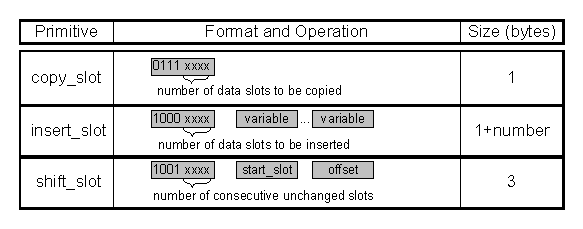
\includegraphics[scale=1.2]{./figures/fopcodedata.eps}
\caption{The data layout patch script primitives.}
\label{fdatascript}
\end{figure}
In order to update the AMC instructions automatically, the offset assignment changes (rather than affected 
instructions) need to be transmitted. 

Figure \ref{fdatascript} lists the {\it data} layout change primitives that are used to specify the memory layout 
change. I only consider the allocation of scalar variables here. Each memory location contains one variable or multiple 
coalesced variables (\cite{related:ottoni,related:zhuang,zhuangtoplas}). 
The old memory layout is maintained on the sensor, and when it receives a update patch with the data layout
changes, it will reconstruct the new memory layout onsite.
Both the old and the new memory layout are maintained as tables. Each row represents the variables that share the same 
memory slot and the rows are ordered by the address of the corresponding memory slot.

\subsubsection{copy\_slot}  Similar as the {\tt copy} primitive in the functional primitive set, this primitive copies 
multiple memory slots from the old memory layout to construct the new memory layout. There are two pointers pointing to 
the active memory slot in the new and old table respectively to accomplish the interpretation of this primitive.

\subsubsection{insert\_var} This primitive adds a list of variables to the active memory slot of the new memory layout 
table.
The insertion can be caused by adding a new variable, or by moving an existing variable from another location. The 
latter implicitly has the variable removed from the old location, which is omitted to keep the script compact. 

\subsubsection{shift\_slot} This primitive represents the case that multiple slots may be grouped and shifted from the 
old memory location to the new memory location. The {\tt shift\_slot} primitive specifies the number of slots that need 
to be shifted, the starting point of the shift, and the shift offset.


\subsection{Sensor-side primitive interpretation}

After receiving the update script, each sensor interprets the {\it data update primitives} to generate the new memory 
layout, and then interprets the {\it functional update primitives} to construct basic blocks by inserting, removing, or 
updating certain instructions on top of the old binary version. The interpreter fixes the addressing mode of each 
instruction in a basic block according to the new memory layout, and then writes the completed block into the flash.


\begin{figure*}[htbp]
\begin{center}
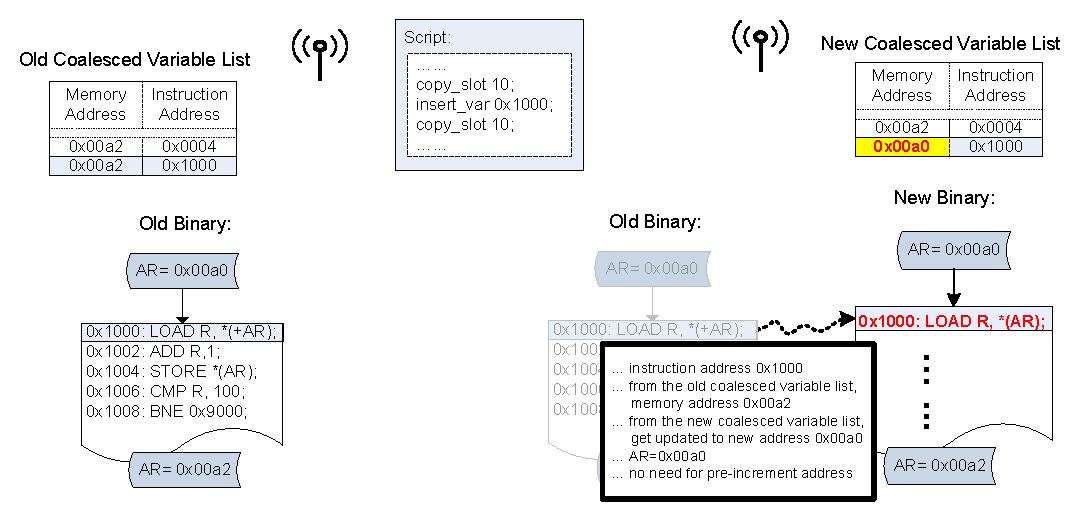
\includegraphics[width=6in]{./figures/correct.eps}
\caption[The code construction procedure of the data primitives.]{The code construction procedure of the data 
primitives.
The left shows the server side, and the right shows the mobile device side updates).}
\label{codecorrection}
\end{center}
\end{figure*}

However, it may require additional information to fix the addressing modes on the mobile device side. As shown in 
Figure \ref{codecorrection}, CSOA coalesces multiple variables --- both {\tt a} and {\tt e}, in one memory location 
{\tt 0x00a2}, a code update may re-allocate {\tt e} to {\tt 0x00a0} while keeping {\tt a} in the same memory slot. This 
complicates the code update as some accesses to {\tt 0x00a0} should be updated while others should not.

Figure \ref{codecorrection} illustrates my solution to this problem. 
I use an implicit pointer to track the current memory slot when copying from the old layout to the new layout.  ``{\tt 
insert\_var} {\tt 0x1000}'' inserts~{\tt e} into the current slot, i.e. {\tt 0x00a0}. Here variable {\tt e} is 
represented using its instruction address {\tt 0x1000}. A record can be found in the coalesced variable list indicating 
this mapping, and will be updated to reflect to the re-allocation.

To update the addressing mode in the new code, a query is sent to the coalesced variable list, from which we know this 
instruction accesses {\tt 0x00a0} instead of {\tt 0x00a2}. Since AR contains {\tt 0x00a0} when entering the basic 
block, there is no need for pre-increment. Similar decisions are made for other instructions in the basic block and 
ensure the exiting AR contains {\tt 0x00a2}.

From this discussion, the interpreter needs the following information to fix the addressing modes:
\begin{itemize}
	\item A coalesced variable list to distinguish each of coalesced variables; and
	\item The AR values when entering and exiting each basic block.
\end{itemize}

\subsubsection{Auxiliary data structures}
To correctly update the code with a memory layout change, e.g. {\tt a} is assigned to a different memory location, we 
need to locate all of {\tt a}'s uses and ensure the AR contains the correct address when accessing {\tt a}. 
Conceptually, this can be done by a relocation table. Unfortunately a traditional relocation table identifies all the 
places that the binary code accesses the memory. Since DSP code relies heavily on offset assignment and accesses the 
memory frequently, adopting a traditional relocation table would generate a table linear to the size of the binary 
code. Instead, I introduce the following two lightweight auxiliary data structures to enable relocatable DSP code.

{\bf Coalesced variable list.}
The coalesced variable list is designed to differentiate the coalesced variables in one memory location. If a memory 
location contains only one variable, then the scheme does not allocate any entry in the list. If multiple variables are 
coalesced and stored in the same memory location, the scheme allocates the entries as follows. 

\begin{figure}[htdp]
\begin{small}
\begin{center}
\begin{tabular}{p{1in} p{1in} }  \hline
Memory  & Instruction  \\
Address & Address \\ \hline\hline
0x00a2 & 0x0004  \\
0x00a2 & 0x1000  \\ \hline
\end{tabular}
\end{center}
\caption{Coalesced variable list.}
\label{memvar}
\end{small}
\end{figure}

Since the coalesced variables have their accesses spread in the code, I group consecutive definitions/uses that access 
the same variable and allocate one entry to each group. This is done based on the code text without considering the 
control flow, or the variable live range etc. For example, if the live ranges of two coalesced variables overlap due to 
linear layout of control structures such as branches, then we allocate one entry for each segment. As shown in 
Figure~\ref{memvar}, each entry contains two fields: the memory slot address, and the starting instruction address of 
each code text segment. 

For example, variable {\tt a} and {\tt e} share the same memory location {\tt 0x00a2}. The live ranges of {\tt a} and 
{\tt e} are {\tt [0x0000,0x0004]} and {\tt [0x0010,0x1000]} respectively. Figure \ref{memvar} illustrates its coalesced 
variable list. Given a memory access to {\tt 0x00a2}, we can easily differentiate whether it is accessing {\tt a} or 
{\tt e}.

The original coalesced variable list is preloaded on the mobile devices before deployment. The updates to the coalesced 
variable list is transmitted with the code update script. The coalesced variable list update primitives will be 
discussed later.

{\bf AR in/out value list.} 
As discussed before, we need the AR in and out values for each basic block in order to generate the correct addressing 
modes on the mobile device side. I choose to construct the list rather than building the control flow graph on demand 
to reduce the memory and complexity overheads. This table contains the starting, ending addresses, the address 
register's entering, exiting values and the successive basic block(s) of each basic block, as shown in Figure 
\ref{bbtable}.

\begin{figure}[htdp]

\begin{center}
\begin{small}
\begin{tabular}{p{0.5in}p{1in}p{1in}p{1in}p{1in}p{1in}}
\hline
Index & Starting  & Ending  & AR In & AR Out & Successive \\
&Address&Address & & &Basic Blocks\\
\hline\hline
10 & 0x1000 & 0x1008 & 0x00a0 & 0x00a2 & 20\\ \hline
\end{tabular}
\end{small}
\end{center}
%\vspace{-0.1in}
\caption{The AR in/out value list.}
\label{bbtable}
%\vspace{-0.1in}
\end{figure}%

The original list is preloaded on the mobile devices before deployment. The interpreter automatically generates the new 
list while generating the new binary code. 

The AR out value of a basic block may affect the addressing mode of its successive basic blocks. The situation becomes 
more complicated if there are multiple predecessors (or successors). Synchronization needs to be done among these 
predecessors (or successors), which may cascadingly affect other instructions in those basic blocks. To simplify the 
code update on mobile device side, the server explicitly sends out the AMC instructions that follow an 
inserted/updated/removed instruction, and those that are the last instruction of a basic block.

{\bf Complexity analysis.}
The following pseudo code Algorithm~\ref{datadecode} presents the algorithm that is used to correct the addressing 
modes based on the data change primitives. The extra interpretation overhead is to look up the address register value 
for the first instruction of each basic block, keep track of this value while constructing the instructions in the 
basic block, and generate the correct addressing mode for each memory access instruction. However, addressing mode 
correction is only necessary 
when the data layout is changed for the corresponding code segment. For example, if the highlighted variable list 
change is the only memory layout change in the example shown in Figure~\ref{codecorrection}, the instructions before 
0x1000 do not need to be decoded, because the memory layout change do not affect those instructions.



\begin{algorithm}
\singlespace
\begin{algorithmic}[1]
\singlespace
\REQUIRE{Instruction {\bf $i$} which will be copied from old binary to the new binary,\\
address of this instruction in the old binary {\bf $addr1$},\\
address of this instruction in the new binary {\bf $addr2$}}
\ENSURE{Instruction $i'$ which has the same opcode as $i$ and with the addressing mode corrected}
	\IF{inst\_type($i$) is memory access instruction}
		\STATE\COMMENT {find out the value stored in address register (AR)}
		\IF{$i$ is the first instruction of basic block $B1$ in old binary}
			\STATE $old\_ar\_value$ = query\_old\_AR\_tab($B1.AR\_in$)
		\ENDIF	
		\IF{$i$ is the first instruction of basic block $B2$ in new binary}
			\STATE $new\_ar\_value$ = query\_new\_AR\_tab($B2.AR\_in$)
		\ENDIF
	\STATE	
	\STATE\COMMENT{find out the memory address that this instruction tries to access}
	\STATE $old\_mem\_addr$ = gen\_addr\_mode($old\_ar\_value$, addr\_mode($i$))
	
	\STATE\COMMENT{find out the variable that this instruction tries to access}
	\STATE $var\_name$ = query\_old\_var\_tab($old\_mem\_addr$, $addr1$)
	
	\STATE\COMMENT{find out the new memory location of this variable}
	\STATE $new\_mem\_addr$ = query\_new\_var\_tab($var\_name$, $addr2$)
	\STATE
	\STATE\COMMENT{generate the new addressing mode and construct the instruction}
	\STATE $addr\_mode$ = form\_addr\_mode($new\_mem\_addr$,$new\_ar\_value$)
	\STATE instruction $i'$ = form\_inst(opcode($i$),$addr\_mode$)
	\STATE return $ i'$
	\ENDIF	
\end{algorithmic}
\caption{{\bf addr\_mode\_correction} /*Correct the addressing mode of an instruction*/}
\label{datadecode}
\end{algorithm}



Each entry of the ``coalesced variable list'' is 4 bytes, and each entry of the ``AR in/out value list'' is 9 bytes,
so they can both fit in the program memory for fast access.
